\documentclass[a4paper,11pt]{report}
\usepackage[french]{babel}
\usepackage[T1]{fontenc}
\usepackage[utf8]{inputenc}
\usepackage{lmodern}
\usepackage{microtype}
\usepackage{hyperref}
\usepackage{tabulary}
\usepackage{framed}
\usepackage{fancyhdr}
\usepackage{amsmath}
\usepackage{bbm}
\usepackage{graphicx}
%\usepackage{pst-all}
%\usepackage{xcolor}
%\usepackage{nopageno}

\newcommand{\latin}[1]{\textit{#1}}

\pagestyle{empty}

\pagestyle{fancy}
\fancyhead{}
\renewcommand{\headrulewidth}{0.5pt}
\fancyhead[R]{\textit{\nouppercase{\rightmark}}}
\fancyfoot{}
\renewcommand{\footrulewidth}{0.5pt}
\fancyfoot[L]{\textit{\nouppercase{\leftmark}}}
\fancyfoot[R]{\thepage}
  
\begin{document}
	\begin{titlepage}
		\vspace*{\stretch{2}}
		\begin{center}
			\large\bfseries\itshape Stage ETE 2015\\
		\end{center}
		\noindent\rule{\linewidth}{3pt}

		\begin{center}
			\Huge\bfseries\itshape Description du système\\
		\end{center}
		
		\noindent\rule{\linewidth}{3pt}
		\begin{center}
			\bfseries
			\large F-PHT \\
			\large Un système d'index de filtres de Bloom pour la recherche d'information par mots clés
		\end{center}
		\vspace*{\stretch{2}}
		\begin{center}
			Réalisé par \textbf{DOAN} Cao Sang \\
			Encadrant: M. \textbf{MAKPANGOU} Mesaac, Regal
		\end{center}
		\vspace*{\stretch{0.5}}
		\begin{center}
			1 Juillet 2015
		\end{center}
	\end{titlepage}

\tableofcontents

\chapter{Vue globale}
\section{Prefix Hash Tree (PHT)}
	Un arbre préfixe est un arbre numérique ordonné qui est utilisé pour stocker une table associative où les clés sont généralement des chaînes de caractères. Contrairement à un arbre binaire de recherche, aucun nœud dans le trie ne stocke la chaîne à laquelle il est associé. C'est la position du nœud dans l'arbre qui détermine la chaîne correspondante\footnote{Wikipédia}.
	
	Pour tout nœud, ses descendants ont en commun le même préfixe. La racine est associée à la chaîne vide. Des valeurs ne sont pas attribuées à chaque nœud, mais uniquement aux feuilles et à certains nœuds internes se trouvant à une position qui désigne l'intégralité d'une chaîne correspondante à une clé.
	
	Pour faire une recherche d'une valeur associée à une clé, au départ, on se situe à la racine de l'arbre, en prenant le premier élément de la clé de la requête, on trouve le chemin étiqueté par cet élément, s'il n'existe pas, on est sûr que cette clé n'est pas dans l'arbre. Dès que l'on trouve le chemin, on arrive sur le bon nœud et continue en prenant le deuxième élément de la clé de requête, on applique cette méthode jusqu'à quand on trouve cette clé et se termine sur une feuille.
	
	\begin{figure}[!htbp]
	\centering
	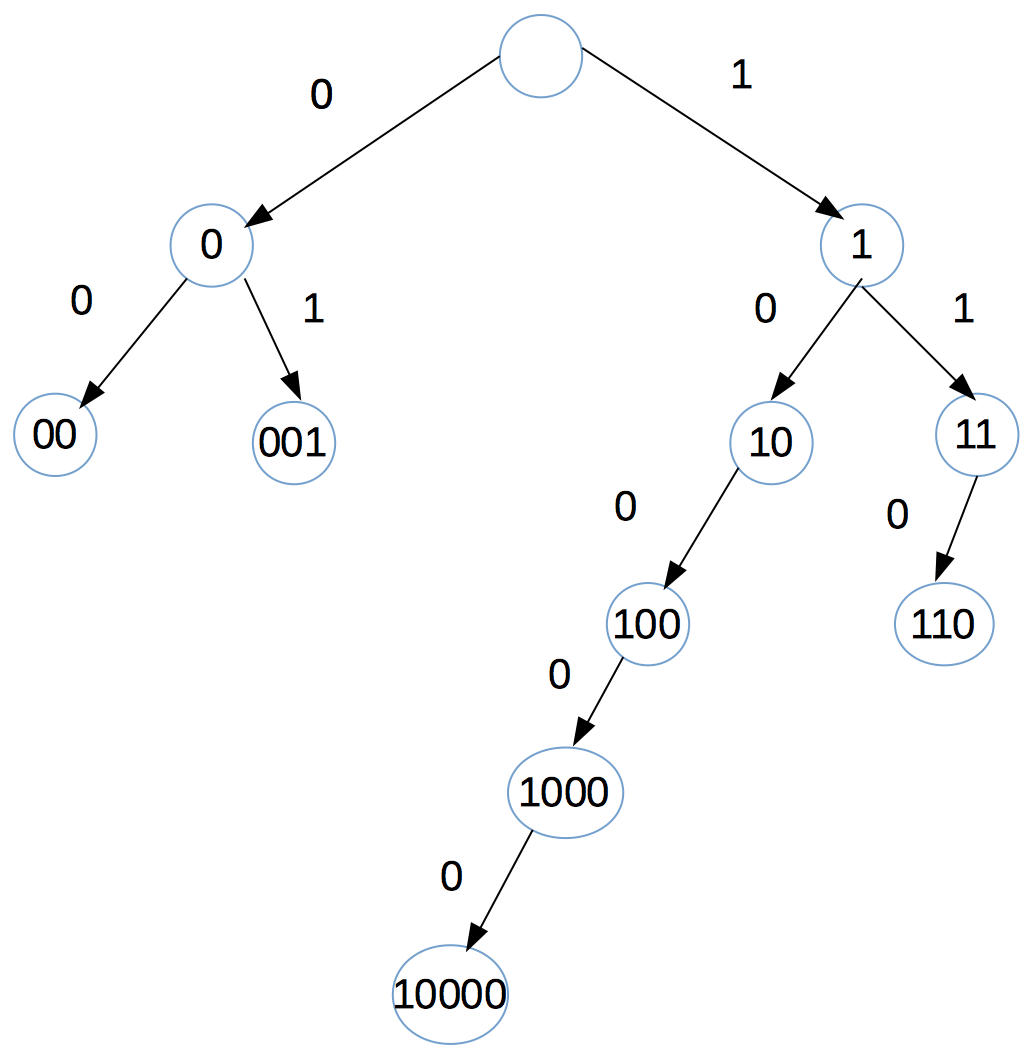
\includegraphics[width=12cm]{PHT.eps}
	\caption{Un arbre de préfixe}
	\label{PHT}
	\end{figure}	

\newpage

\section{Fragment}
	On considère un filtre de Bloom de taille \textit{m}. Le système découpe ce filtre en \textit{f} fragments de taille identique. Par convention, ces fragments sont numérotés de \textit{0} à \textit{f-1}, en commençant par le fragment le plus à gauche. L'identifiant de chaque fragment est défini de façon unique.
	
		Par exemple, un filtre de Bloom de taille \textit{m = 16} bits, il s'est découpé en \textit{f = 4} fragments, donc chaque fragment est de taille $a = \frac{m}{f} = 4$ bits.

	\begin{table}[!h]
		\centering		
		\begin{tabular}{|l|*{14}{c|}r|}
		\multicolumn{1}{c}{{\scriptsize 15}} &\multicolumn{1}{c}{}&\multicolumn{1}{c}{}&\multicolumn{1}{c}{}&
		\multicolumn{1}{c}{}&\multicolumn{1}{c}{}&\multicolumn{1}{c}{}&\multicolumn{1}{c}{}&
		\multicolumn{1}{c}{}&\multicolumn{1}{c}{}&\multicolumn{1}{c}{}&\multicolumn{1}{c}{}&
		\multicolumn{1}{c}{}&\multicolumn{1}{c}{}&\multicolumn{1}{c}{}&\multicolumn{1}{c}{{\scriptsize 0}}\\
		\hline
			1 & 0 & 0 & \multicolumn{1}{c||}{0} & 
			1 & 1 & 0 & \multicolumn{1}{c||}{1} & 
			0 & 0 & 0 & \multicolumn{1}{c||}{0} & 
			1 & 0 & 1 & 0 \\
		\hline
		\end{tabular}
		\caption{Exemple le filtre de Bloom}
		\label{fragment/filtredeBloom}
	\end{table}

	\begin{table}[!h]
		\centering		
		\begin{tabular}{|l|*{2}{c|}r|}
		\hline
			1 & 0 & 0 & 0 \\
		\hline
		\end{tabular}
		\caption{Exemple la valeur de fragment \textit{0}}
		\label{fragement/exemple1}
	\end{table}

	\begin{table}[!h]
		\centering
		\begin{tabular}{|l|c|c|r|}
		\multicolumn{1}{c}{}&\multicolumn{1}{c}{}&\multicolumn{1}{c}{}\\
		\hline
			1 & 0 & 1 & 0 \\
		\hline
		\end{tabular}
		\caption{Exemple la valeur de fragment \textit{3}}
		\label{fragement/exemple2}
	\end{table}
	
\section{F-PHT}
	F-PHT est une sorte d'arbre préfixe, il utilise  les filtres de Bloom  de taille \textit{m} comme clés de stockage. Cet arbre utilise la valeur d'un fragment de filtre de Bloom de rang \textit{i} à la place de préfixe. Chaque nœud de l'arbre stocke un ensemble de couple \textit{<R, id\_R>} avec \textit{R} est la valeur d'un fragment de rang \textit{i} et \textit{id\_R} est soit l'identifiant d'un nœud, soit \textit{null}. Si \textit{id\_R} est égal à \textit{null}, \textit{R} est un filtre de Bloom. Sinon, ce couple désigne où sont stockés les filtres de Bloom ayant \textit{R} comme valeur du fragment de rang \textit{i}, où \textit{i} correspond au niveau de ce nœud dans l'arbre.

	Chaque nœud de rang \textit{i} contient une table \textit{RouteEntry}, qui contient les couples stockés par ce nœud. Chaque nœud stocke au plus $\gamma$ couples, avec $\gamma \leq 2^{\frac{m}{f}}$. A l'initialisation du système, cette table est vide, elle sont remplit au fur et à mesure automatiquement. Une fois, la capacité a été débordée, le système éclate ce nœud en créant des nouveaux fils de rang \textit{i+1} et met à jour la table \textit{RouteEntry}.
	
	Dans cette exemple, nous montrons un F-PHT avec le filtre de Bloom de taille \textit{m = 6} bits, découpé en \textit{f = 3} fragments de taille \textit{a = 2} bits, chaque nœud contient au maximum $\gamma = 2^{2}$ éléments.
	
	\begin{figure}[!htbp]
	\centering
	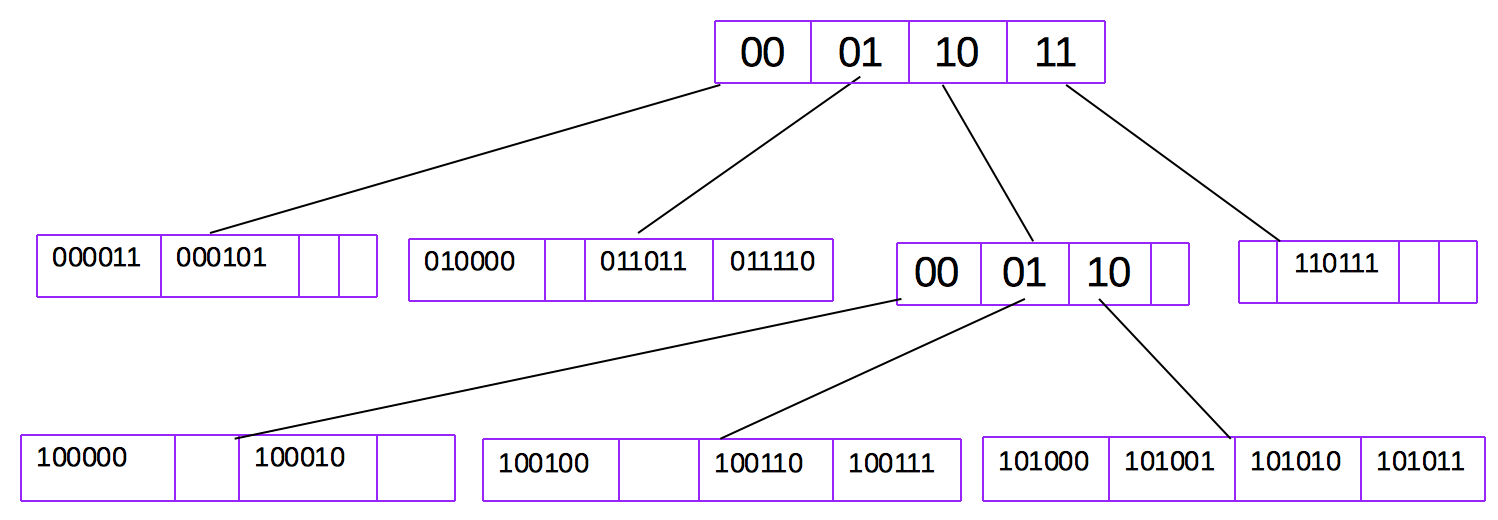
\includegraphics[width=15cm]{F-PHT.eps}
	\caption{La vue logique du système de F-PHT}
	\label{F-PHT}
	\end{figure}	
	
\chapter{Système d'indexation}
	Le système d'indexation est un système qui indexe les données pour faciliter la recherche de données, il gère en général une très grande quantité de données. Il existe plusieurs façon d'indexation des données comme table de hachage distribuée, arbre binaire, arbre de préfixe... Mais le problème est que le plupart des techniques sont destinés à la recherche exacte, c-à-d que le résultat obtenu est une chose précise et exactement égal à la requête.
	
	Reprenez la figure \ref{PHT}, on veut chercher un mot qui se termine par "000", cette technique doit obligatoirement chercher tous les chemins en descendant jusqu'à chaque feuille. Elle est incapable de réduire le nombre de chemins qui ont fortement de chance de trouver le résultat. 
	
	Dans le cadre de mon travail, ce système arrange les données dans un arbre F-PHT en utilisant le filtre de Bloom pour générer les clés de stockage et aussi les données. F-PHT est une évaluation de son frère PHT, nous permet de chercher moins de chemins sans laisser passer aucun élément.
	
	Ce système dispose les actions principales comme:
	\begin{itemize}
		\item Ajout d'un filtre de Bloom dans le système.
		\item Recherche des filtres de Bloom.
		\item Suppression d'un filtre de Bloom.
	\end{itemize}
	
\section{Ajout d'un filtre de Bloom dans F-PHT}
	Comme le F-PHT utilise des fragments d'un filtre de Bloom comme clés de stockage, le système crée un fragment \textit{$R_i$} de rang \textit{i}, au départ \textit{i = 0} comme le rang de la racine. Ensuite, à partir de ce fragment, un couple \textit{<$R_i$, null>} est soumit à la racine pour ajout dans l'arbre. La façon de traitement dans chaque nœud dépend la nature de ce nœud, soit un nœud soit une feuille.

\subsection{Cas d'un nœud feuille de rang i dans F-PHT}
	Tant que la capacité de la table \textit{RouteEntry} qui stocke les couples terminaux \textit{<R, null>} dans ce nœud feuille est inférieure à $\gamma$, chaque nouveau couple terminal qui arrive sur ce nœud feuille est simplement ajouté dans \textit{RouteEntry}.

	Une fois, la capacité de cette table atteinte, elle ne peut plus stocker des nouveaux couples qui arrivent. Donc, dans ce cas, le nœud feuille exécute une opération interne du système d'indexation pour qu'elle puisse les ajouter. \textbf{split()} est une opération utilisée lors que le système veut éclater un nœud, les étapes sont:
	\begin{enumerate}
		\item Le système crée une nouvelle instance de \textit{RouteEntry} initialisée à vide.
		\item Le système regroupe tous les éléments qui ont la même valeur de fragment de rang \textit{i+1} \textit{$R_{i+1}$}, cette valeur est calculée à partir du couple terminaux dans l'ancienne table \textit{RouteEntry}.
		\item Pour chaque valeur différente de fragment trouvée, le système crée un nœud fils qui a l'identifiant \textit{id\_$R_{i+1}$} unique calculé à partir de \textit{$R_{i+1}$} et lui transfère l'ensemble des éléments qui ont même \textit{$R_{i+1}$}, puis ajoute le couple \textit{<$R_{i+1}$, id\_$R_{i+1}$>} dans la nouvelle table \textit{RouteEntry}.
		\item Une fois tous les nœuds fils crées et les couples terminaux sont transférés vers les fils correspondants, l'ancienne table \textit{RouteEntry} est remplacé par cette nouvelle.
		\item Enfin, le système traite la nouvelle demande.
	\end{enumerate}
	
\subsection{Cas d'un nœud interne de rang i dans F-PHT}
	Lorsqu'un nœud interne reçoit un couple terminal \textit{<R, null>}, le système vérifie si le fragment de rang \textit{i} \textit{$R_{i}$} de ce couple est égal au sien, sinon, il jette ce couple. Si oui, il calcul le fragment de rang \textit{i+1} \textit{$R_{i+1}$} de ce couple et cherche dans sa propre table \textit{RouteEntry}, s'il existe un fils qui gère les couples de ce fragment, il lui envoie ce couple terminal. S'il n'existe pas dans la table, le systèmre crée le nœud fils qui a l'identifiant \textit{id\_$R_{i+1}$} calculé automatiquement à partir de \textit{$R_{i+1}$} et ajoute le couple \textit{<\textit{$R_{i+1}$}, \textit{id\_$R_{i+1}$}>} dans sa table \textit{RouteEntry}, puis route le couple terminal vers  le fils qui vient d'être créé.
	
\section{Recherche des filtres de Bloom dans F-PHT}
	On considère que la requête \textit{Q}, un filtre de Bloom de taille identique avec ceux qui sont stockés dans F-PHT. Le système doit trouver tous les filtres stockés qui satisfont la requête \textit{Q}, c-à-d les filtres qui ont fortement de chance d'avoir les mots de la requête dans leur description. Les faux positifs sont inévitables.
	
	La requête de recherche doit s'adresser à la racine de F-PHT. Chaque nœud commence par déterminer sa nature s'il est un nœud interne ou un nœud  feuille  après la réception de la requête. Car comme l'ajout d'un filtre dans F-PHT, la nature de nœud décide la méthode de traitement de la requête.
	
\subsection{Cas d'un nœud feuille de rang i dans F-PHT}
	Dès qu'un nœud feuille reçoit la requête \textit{Q}, son rôle est de parcourir sa propre table \textit{RouteEntry}, pour chaque couple \textit{<R, null>} il examine si $Q \in R$, s'il y a succès, le nœud ajoute \textit{R} dans l'ensemble de réponses. Après le parcours de \textit{RouteEntry}, il renvoie cet ensemble au père même s'il est vide.
	
\subsection{Cas d'un nœud interne de rang i dans F-PHT}
	Quand un nœud interne reçoit la requête \textit{Q}, le système fait :
	\begin{enumerate}
		\item D'abord, il détermine la valeur de fragment de rang \textit{i} de la requête \textit{$Q_i$}. Si ce nœud contient probablement la requête, il continue, sinon il renvoie \textit{null} au nœud père.
		\item Ensuite, il détermine la valeur de fragment de rang \textit{i+1} de la requête \textit{$Q_{i+1}$}.
		\item Puis, il examine la table \textit{RouteEntry}, pour chaque couple \textit{<R, id\_R>}, si $Q_{i+1} \in R$, il transfère la requête au fils qui a l'identifiant \textit{id\_R}.
		\item Après la réception de la réponse de tous ses fils auxquels il l'ont envoyé, il rassemble toutes les réponses et répond au nœud père. Donc, à la fin, la racine a reçu le résultat final de la requête.
	\end{enumerate}
	
\section{Suppression d'un filtre de Bloom de F-PHT}
	Afin de supprimer un filtre de Bloom dans F-PHT, le système exécute une recherche exacte en prenant ce filtre comme la requête \textit{Q}. Il faut trouver exactement le nœud feuille qui stocke cette requête, il doit d'abord calculer le fragment de la requête au rang \textit{i} \textit{$Q_i$}. Ensuite, le nœud interne de rang \textit{i} qui a sa propre valeur de fragment de rang \textit{i} qui est identique avec \textit{$Q_i$} est chargé de chercher dans sa propre table \textit{RouteEntry} le fils qui gère le fragment de rang \textit{i+1} et sa valeur est égale à celle de la requête \textit{$Q_{i+1}$}. S'il n'a pas trouvé, cela veut dire qu'il n'existe pas ce filtre de Bloom dans F-PHT. Sinon, il transfère cette requête à ce fils.
	
	Une fois, on trouve la feuille qui stocke la requête \textit{Q}, elle peut trouver facilement dans sa table \textit{RouteEntry} et supprime le couple qui satisfait la requête. A la fin, en regardant la table, si c'est vide, elle demande le système de détruire ce nœud feuille et elle signale le père que ce fils n'existe plus dans l'arbre. Une fois, le père constate que son fils n'existe plus, il supprime le couple de valeur correspondante dans sa propre table \textit{RouteEntry}. Si après la suppression, cette table est vide, ce nœud demande le système de le détruire et notifier son père. Ce procédure continue jusqu'à quand il n'y a pas une table \textit{RouteEntry} vide.
	
\chapter{Architecture d'un système d'indexation}

	Le système que nous avons décrit ci-dessus est une vue logique à l'extérieur. En réalité, ce système est réparti sur plusieurs sites, sur un réseau pair-à-pair. Mais un site joue le rôle de la racine, par conséquence, tous les autres le connaissent.
	
	\begin{figure}[!htbp]
	\centering
	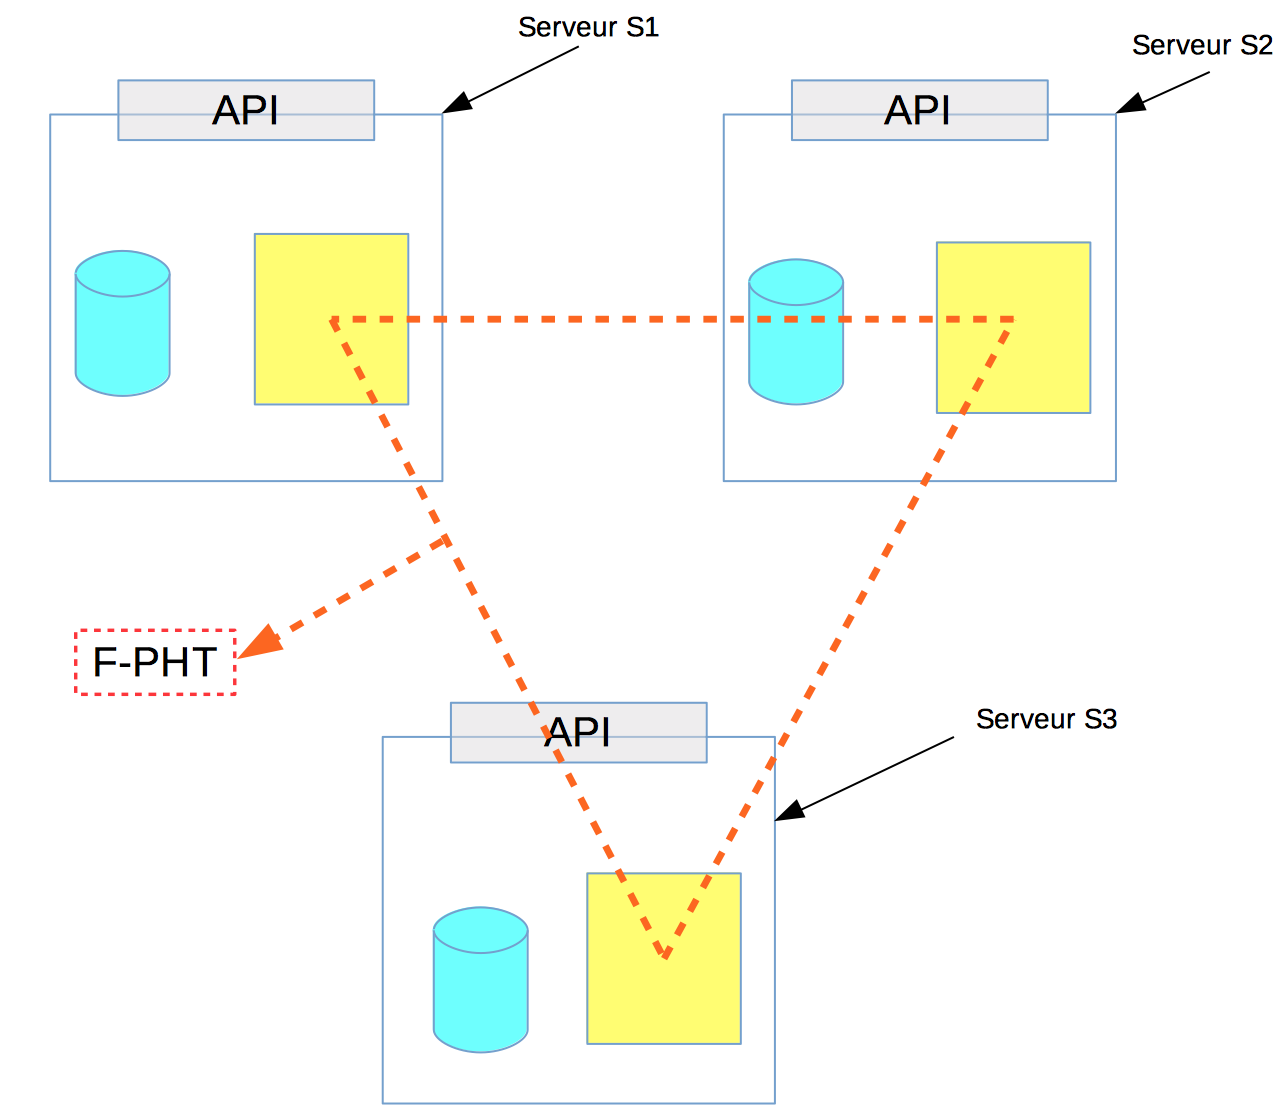
\includegraphics[width=14cm]{systeme-F-PHT.eps}
	\caption{Un système de F-PHT}
	\label{systemeF-PHT}
	\end{figure}	
	
\newpage

	Un site munie une interface API pour faciliter la communication avec l'utilisateur, un endroit où il stocke les données \textit{DataStore} et un système d'indexation. Le \textit{DataStore} stocke les documents avec leurs descriptions, nous n'entrons pas au détail dans notre travail. Tous les sites implémentent un même système d'indexation et se communiquent via le réseau.
	
\end{document}









